\chapter{Synchronization}
\label{sync-chapter}

LSDj can synchronize with other devices through the link port, so that it is possible to run both in exactly the same tempo. Enable synchronization by changing the \textsc{sync} mode in the project screen.

\textsc{Important}: When running synchronized, use a groove based on 6 ticks/step. Otherwise, the resulting speed might be wrong.

\section{Game Boy to Game Boy Sync}

It is possible to sync two Game Boys running LSDj using a Nintendo Game Link cable.

\subsection{Activating LSDj Sync}

Make sure that both Game Boys are turned off. Connect the Game Boys using the link cable. Now, turn on the Game Boys, and go to the project screens. Set the \textsc{sync} mode to \textsc{lsdj} on both Game Boys.

\subsection{Song Play}

When in song mode, pressing \textsc{start} starts both Game Boys from the same song position. The Game Boy on which you pressed \textsc{start} is the one that sends sync signals; this is indicated by the text \textsc{lead} appearing in the right margin. The other Game Boy shows the text \textsc{sync}, indicating that it is receiving sync signals.

\subsection{Live Play}

Pressing \textsc{start} in live mode makes the Game Boy start like usual; also \textsc{lead}/\textsc{sync} texts indicate that sync signals are sent between the Game Boys. When pressing \textsc{start} on the following Game Boy, the text \textsc{wait} appears while it is waiting for a phrase start.

\subsection{Clipboard Transfer}

When two Game Boys are linked and not playing, copying groove, chain, phrase, instr, table or synth data on one Game Boy will transfer the copied data so it can be pasted on the other Game Boy.

\subsection{Switching Lead while Playing}

In some cases, it can be useful to switch which Game Boy is the lead while playing. Do this by following steps:

\begin{enumerate}
    \item Set Game Boys to \textsc{lsdj} sync.
    \item Start playing.
    \item Set the following Game Boy to sync \textsc{off}.
    \item Stop lead Game Boy.
    \item Set the following Game Boy to sync \textsc{lsdj}. It now becomes the lead.
\end{enumerate}

\section{\textsc{Midi} Sync}

\textsc{Midi} sync requires a special \textsc{Midi} sync cable for Game Boy. For information on how to build a \textsc{Midi} to Game Boy adapter, please refer to the website at \url{https://www.littlesounddj.com}.

Usage: Plug in the sync device before turning on your Game Boy. Then, set LSDj to \textsc{Midi} sync mode. Pressing \textsc{start} will now make LSDj wait for and sync with any incoming \textsc{Midi} clock signals. LSDj should use grooves based on 6 ticks.

\begin{figure}[hbtp]

\includegraphics[width=0.84cm]{tip}TIP!
\begin{itemize}
        \item \textit{When LSDj is following, it is possible to temporarily play
slower or faster by pressing \textsc{a+left/right} on tempo in project screen. This can
be very useful when being hooked up to some external hardware that has drifted slightly out
of sync.}
	\end{itemize}
\end{figure}

\section{Analog In}

LSDj can sync to music equipment that sends analog sync signals. This sync mode has been tested with the Korg Volca series, but works with other gear too; you can find a list at \url{https://littlesounddj.wikia.com/wiki/Analog_Sync_Compatibility}.

A cable should be easy to make, since no particular electronics are needed: all it takes is to splice a Nintendo Game Link Cable and a 3.5 mm mini plug cable together. The wires should be connected as shown in the below diagram: GND goes to GND, CLK goes to CLK.

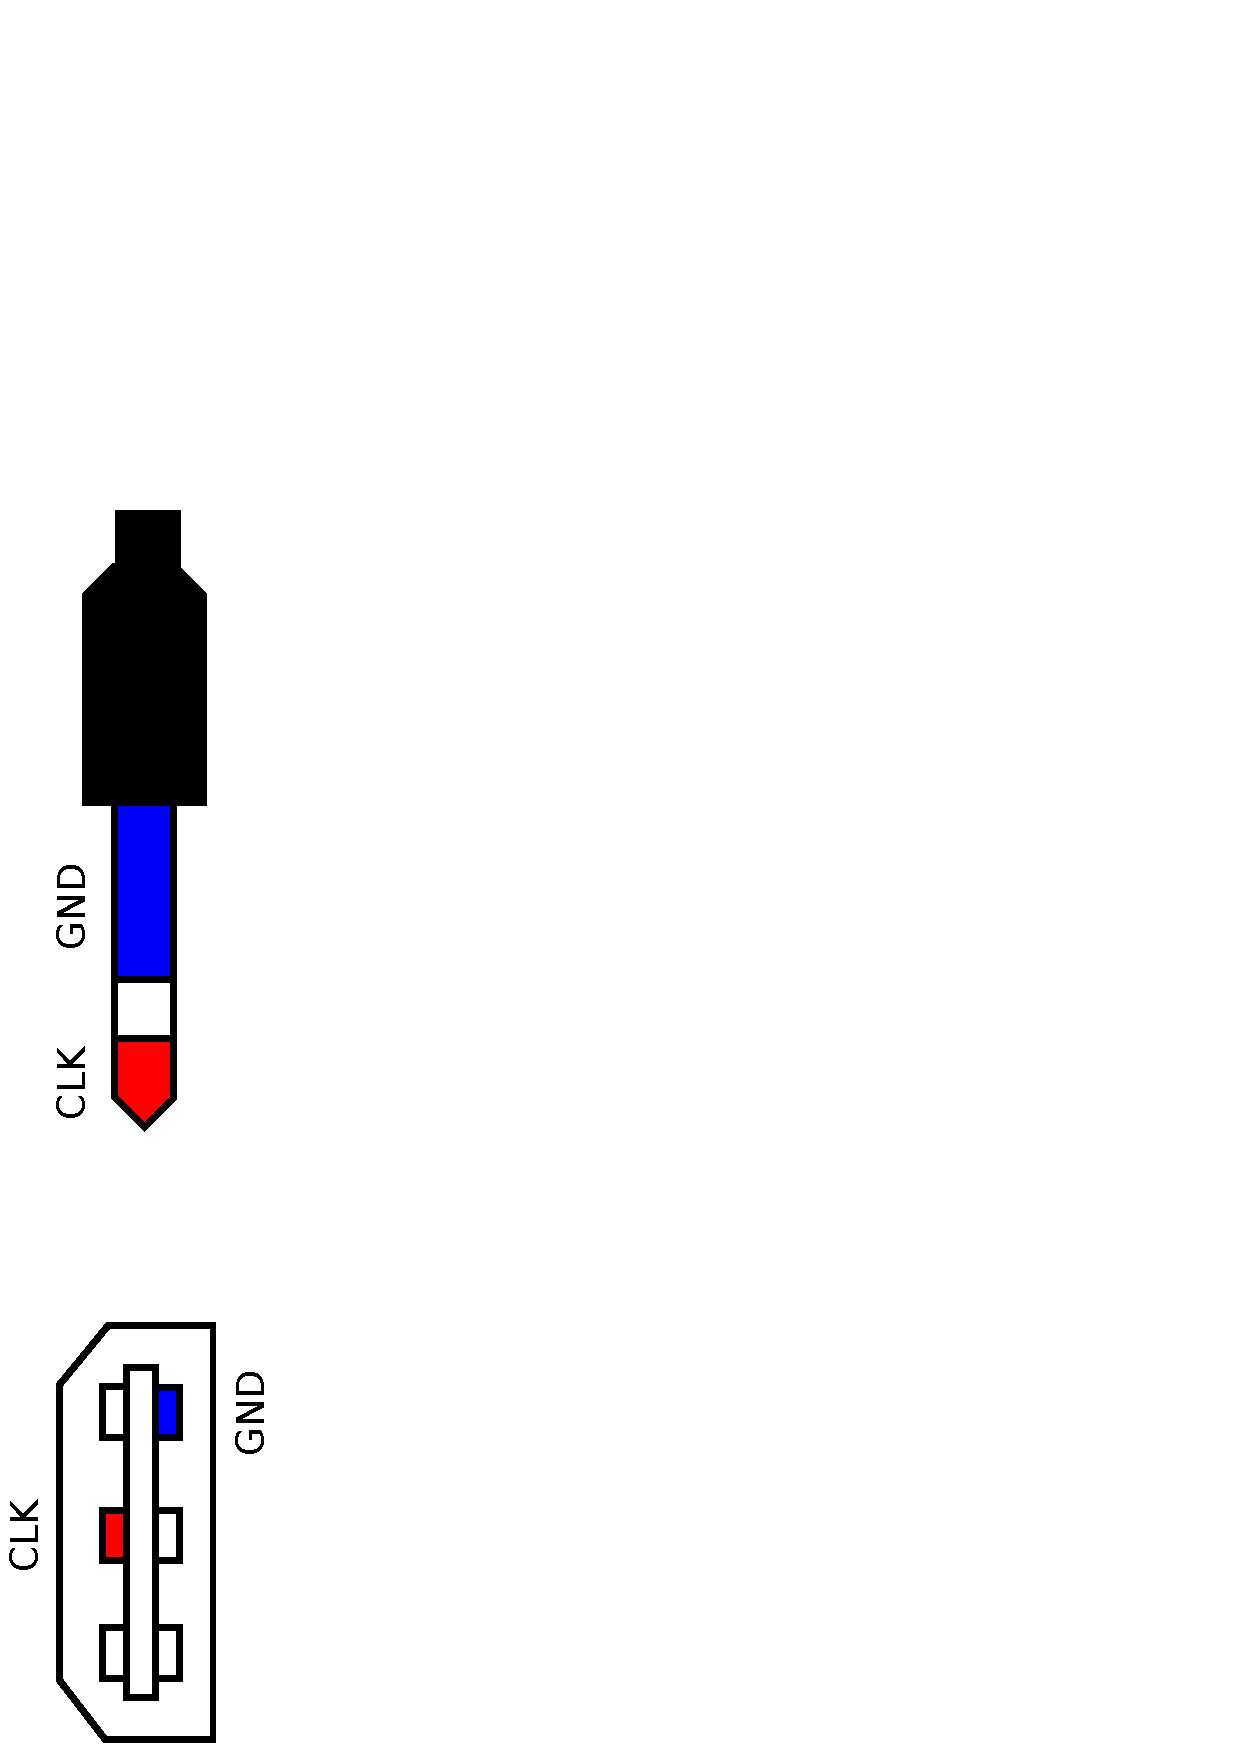
\includegraphics[clip=true,trim=0 0 460 250,angle=270,width=10cm]{analog-in}\\

As a clarification, the above diagram is looking at the cable, and the wires are probably not red and blue in reality.

Once the cable is built, connect it to the Game Boy serial port and the \textsc{sync out} of your synthesizer. In project screen, set LSDj to \textsc{analog} sync mode. The \textsc{ticks/step} setting controls how many LSDj ticks should be generated for each incoming sync signal. Depending on the synthesizer, it may be necessary to change this setting to make LSDj run at the right speed. For Korg Monotribe, it should typically be set to 6, whereas for Korg Volca, it should be C.

\section{Analog Out}

Analog Out works similar to Analog In, except that in this mode, LSDj is responsible for sending the sync signal. The cable is different from the one used for Analog In. Build it by connecting the wires as follows:

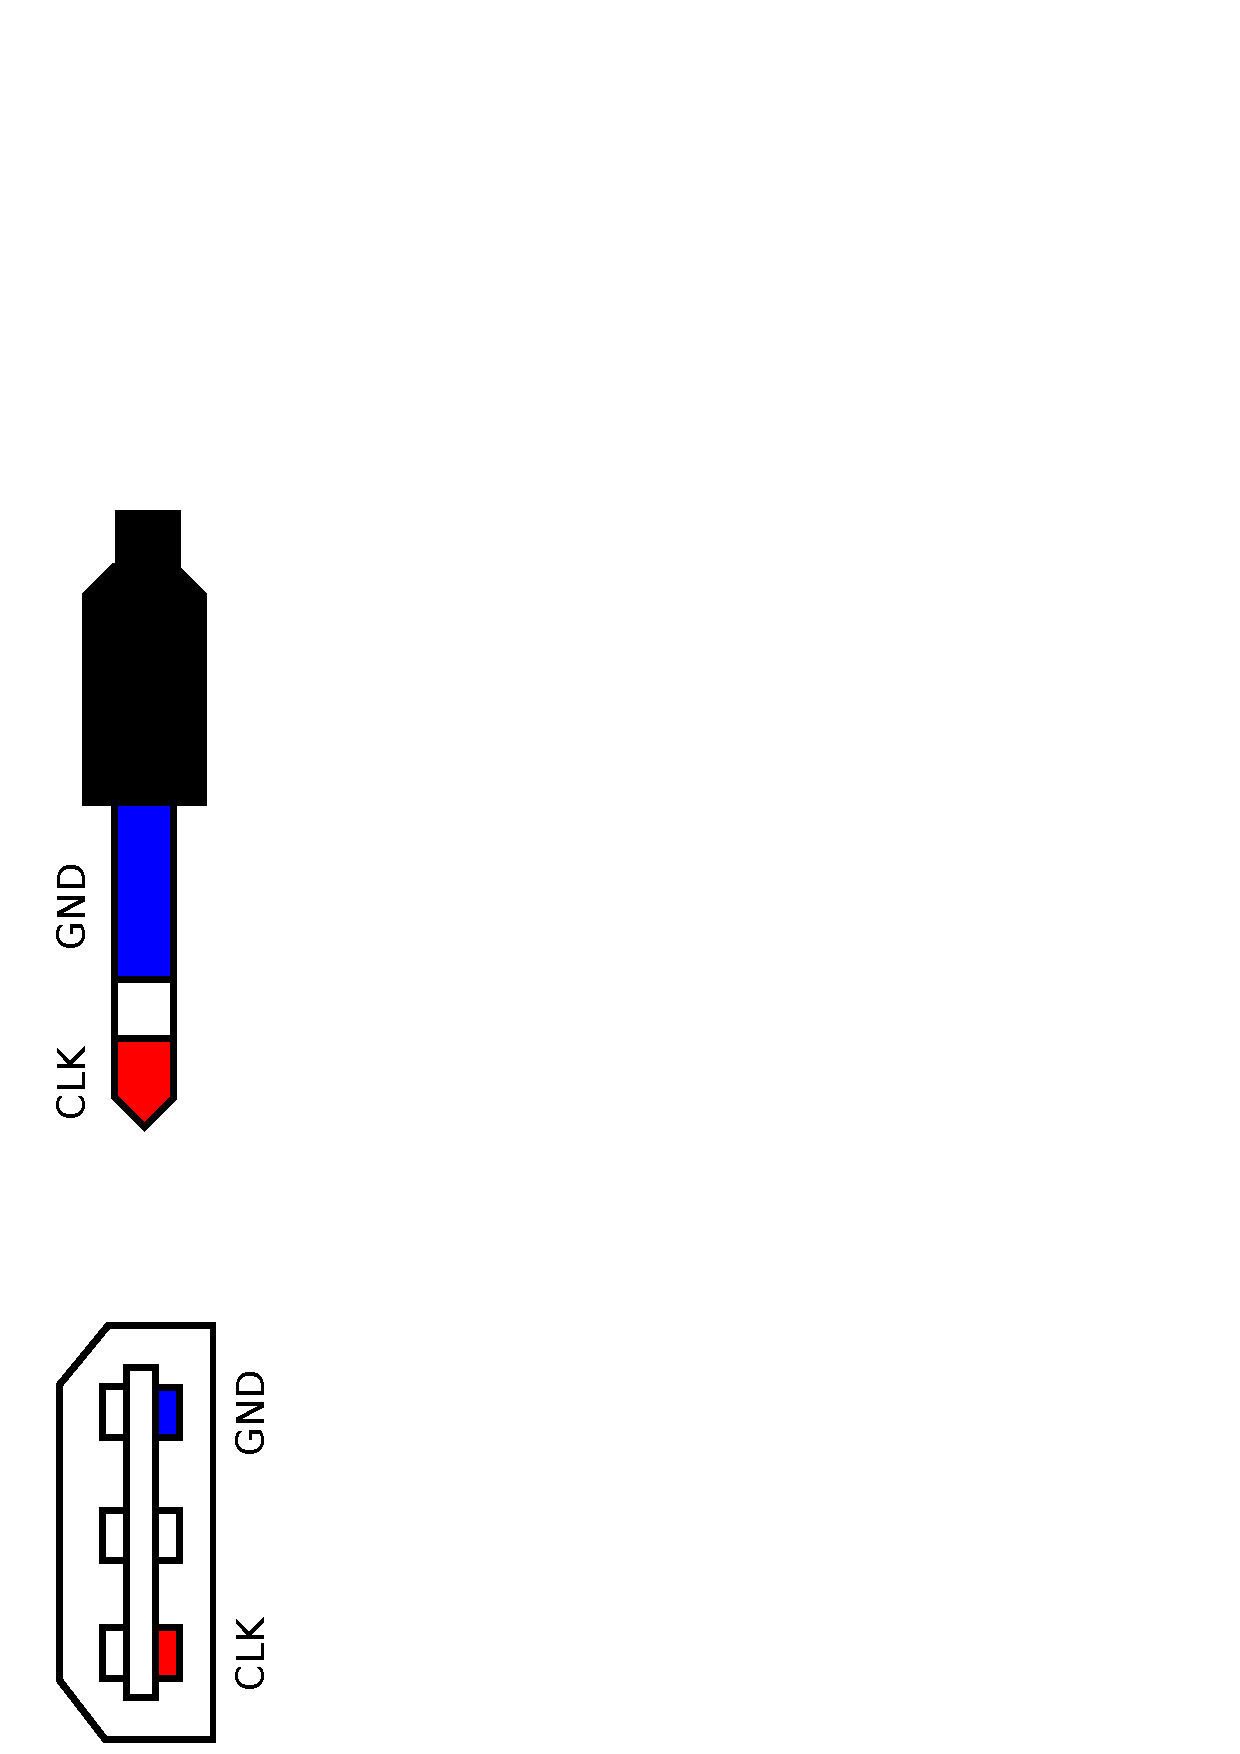
\includegraphics[clip=true,trim=0 0 460 250,angle=270,width=10cm]{analog-out}\\

As a clarification, the above diagram is looking at the cable, and the wires are probably not red and blue in reality. This cable should be connected to \textsc{sync in} of your synthesizer.

\section{Troubleshooting Cables}

When making cables, double and triple check that the wires are connected to the right pins. You will need a multimeter for probing the pins. If they are not connected exactly like they should, you can get cables that nearly work, but the sync is a little off. The most common problem is flipped pins; remember that the diagrams are looking at the cable, not from it!

\section{Keyboard Control}

The \textsc{keybd} sync mode allows connecting a PS/2 keyboard to the Game Boy and playing it like a piano. This can be fun for live shows and improvisation. For information on how to build a PS/2 keyboard to Game Boy adapter, please refer to the Wiki site: \url{https://wiki.littlesounddj.com}

The keyboard must be calibrated once is plugged in. To do this, go to the project screen, set sync mode to \textsc{keybd}, and press \textsc{A} on the \textsc{ps/2 delay} setting. Then, press the down arrow key on your PS/2 keyboard repeatedly until LSDj says \textsc{ok!}

To get sound when playing the keyboard, first go to phrase screen and move cursor to note column, or press \textsc{start} to play the keyboard while the song is running.

\subsection{Keyboard Note Layout}

\begin{figure}[htpb]
	\begin{center}
	\fbox{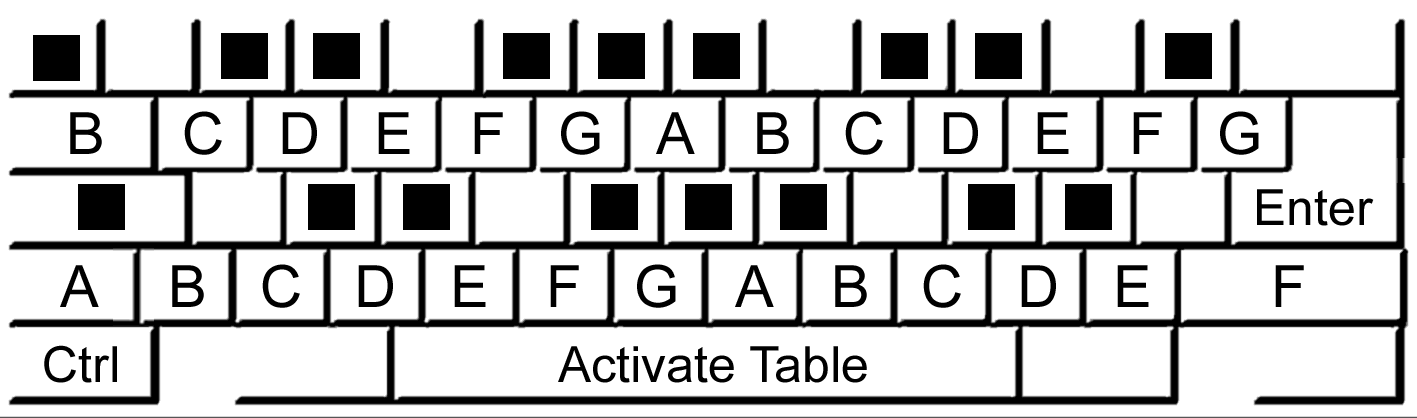
\includegraphics[width=10cm]{keybd-map}}
	\end{center}
	\caption{PC Keyboard Map}
	\label{fig:keybd-map}
\end{figure}

\begin{description}
\item[\textsc{space}] play using custom table
\item[\textsc{f1/f2}] octave down/up
\item[\textsc{f3/f4}] instrument down/up
\item[\textsc{f5/f6}] select custom table to assign to \textsc{space}
\item[\textsc{f8}] change pulse instrument playback channels (\textsc{PU1, PU2, PU1+2})
\item[\textsc{f9-f12}] toggle channel mute (switches on key press)
\item[\textsc{ctrl+(f9-f12)}] tap channel mute (switches on key press and release)
\item[\textsc{cursor movement keys}] move around cursor
\item[\textsc{enter}] play chain
\item[\textsc{ctrl+enter}] stop chain
\item[\textsc{page up/down}] \textsc{b+up/down}
\end{description}

